%%!TEX TS-program = pdflatexmk
%%!TEX encoding = UTF-8 Unicode
\documentclass[11pt]{article}
\usepackage[utf8]{inputenc}
\usepackage[letterpaper,body={6.0in,9.5in},vmarginratio=1:1]{geometry}
\usepackage[small,compact]{titlesec}

\usepackage{fourier}
\usepackage[scaled=0.85]{berasans}
\usepackage[scaled=0.85]{beramono}
\usepackage{microtype}

\usepackage{graphicx}
\usepackage{booktabs}

\usepackage{xcolor}
\usepackage[colorlinks, urlcolor=darkgray, linkcolor=darkgray]{hyperref}

\newcommand{\optkey}{\textsf{Opt}}
\newcommand{\ctlkey}{\textsf{Ctl}}
\newcommand{\cmdkey}{\textsf{Cmd}}
\newcommand{\esckey}{\textsf{Esc}}
\newcommand{\tabkey}{\textsf{Tab}}
\newcommand{\shiftkey}{\textsf{Shift}}

\newcommand{\mnu}[1]{\textsf{#1}}
\newcommand{\cmd}[1]{\textsf{#1}}
\newcommand{\To}{\,\(\to\)\,}

\pagestyle{plain}

\newcommand{\MacTeX}{Mac\kern-.13em\TeX}
\newcommand{\BibTeX}{B\textsc{i\kern-.025em  b}\kern-.13em\TeX}
\newcommand{\TS}{\textsf{\TeX Shop}}

\title{Using \texttt{latexmk} with \TS}
%\author{by\\Herbert Schulz\\\small\href{mailto:herbs2@mac.com}{herbs2@mac.com}}
\author{Herbert Schulz\\\small\href{mailto:herbs2@mac.com}{herbs2@mac.com}}
\date{}

\begin{document}
\maketitle
\thispagestyle{empty}
\section{What is \texttt{latexmk}?}
Compiling a \texttt{tex} file containing cross-references, bibliographic references and/or indexes is a multi-pass process; i.e., you've got to run \texttt{(pdf/xe)latex} multiple times with possible intermediate runs of \texttt{bibtex} and/or \texttt{makeindex} until all references are resolved. The \texttt{latexmk} \texttt{perl} program, rewritten and presently maintained by John Collins\footnote{The \texttt{latexmk} web site is <\url{http://www.phys.psu.edu/~collins/software/latexmk-jcc/}>. You can get the latest version of \texttt{latexmk} at <\url{http://www.phys.psu.edu/~collins/software/latexmk-jcc/versions.html}>. }, automates this multi-pass process. By default it first runs \texttt{(pdf/xe)latex} on a source file, determines file dependencies by examining the \texttt{log} and \texttt{aux} files produced by the run and then automatically runs \texttt{bibtex}\footnote{As of version 4.22 \texttt{latexmk} will automatically choose between running \texttt{bibtex} or \texttt{biber} as required.} and/or \texttt{makeindex}, if needed, and the correct number of additional runs of \texttt{(pdf/xe)latex} to generate the bibliography, index and cross-references. Recent versions of \texttt{latexmk} also work correctly with the \texttt{nomencl} package as well as the  \texttt{glossary} and \texttt{glossaries} packages and other packages that produce multiple bibliographies or indexes.

\section{Quick Start!}

This section will get you started quickly. Unless you are trying to customize the behavior of the supplied engines or want to use the more esoteric engines this really is all you need!

\subsection{Quick Install.}

To activate the \texttt{latexmk} \texttt{engine} files simply move all the files with extension \texttt{.engine} from \path{~/Library/TeXShop/Engines/Inactive/Latexmk/} two folder levels up, to \path{~/Library/TeXShop/Engines/}, and (re-)start \TS. (Note: \path{~/Library/} is the \cmd{Library} folder in your \cmd{HOME} folder.) When you click on the popup engine menu on the Source toolbar the newly enables engines names should appear; see Figure (\ref{fig:popupmenus}) to see how that menu changes. \textbf{Note: the engine names will \emph{not} appear in the \texttt{Typeset} Menu.}

\subsection{Quick Use.}

At the top of your Source file place the line
\begin{verbatim}
% !TEX TS-program = pdflatexmk
\end{verbatim}
to use the \texttt{pdflatexmk} engine which will use \texttt{pdflatex} to typeset your document. Substitute \texttt{latexmk} or \texttt{xelatexmk} for \texttt{pdflatexmk} to use \texttt{latex} or \texttt{xelatex} to typeset your Source. From then simply using \texttt{Typeset}\(\to\)\texttt{Typeset} (\texttt{Cmd-T}) will run through the complete process of fully typesetting your document.

\section{What is here?}

There is a set of nine \texttt{engine} files to be placed in \path{~/Library/TeXShop/Engines/}. There is a \texttt{tslatexmk} folder already placed in \path{~/Library/TeXShop/bin/}. The files in that folder consist of the \texttt{latexmk} program, nine basic initialization (\texttt{rc}) files used by the nine \texttt{engine} files, a common file for personal settings (\texttt{latexmkrcDONTedit}) and two shell scripts used for \texttt{pdftricks} and \texttt{pst-pdf} figure processing. When any of the new engines is first run the \texttt{latexmkrcDONTedit} file will automatically be copied to \path{~/Library/TeXShop/bin/latexmkrcedit} if it doesn't already exist. You may copy the file there manually if you wish. \textbf{Any changes or additions to the configuration (e.g., new dependencies and rules) should be placed in the \texttt{laxtexmkrcedit} file. When \TS\ is updated the files in the \path{~/Library/TeXShop/bin/tslatexmk} may automatically get updated; don't edit them or your changes may get lost.}

\section{Using \texttt{latexmk} with \TS.}

\textbf{NOTE: If you are updating to this version of \texttt{latexmk} for \TS\ from a previous version you need only activate the engine files, as noted above, and restart \TS\ after installing the files.
%(You should also remove \texttt{makeglos.pl} and \texttt{makeglossaries} from  \path{~/Library/TeXShop/bin/} if they were installed with a previous version of \texttt{latexmk} for \TS\ since they are no longer used.)
}


There are nine \texttt{engine} files; two for running \texttt{latex} (one with a final run through \texttt{dvips} and \texttt{ps2pdf} [\texttt{latexmk.engine}] and one with a final run through \texttt{dvipdfmx} [\texttt{dvipdfmxmk.engine]}), one for using \texttt{pdflatex} [\texttt{pdflatexmk.engine}], one for using \texttt{xelatex} [\texttt{xelatexmk.engine}], one for using \texttt{lulatex} [\texttt{lulatexmk.engine}], two for using the \texttt{pdftricks} or \texttt{pst-pdf} packages with \texttt{pdflatex} [\texttt{pdftricksmk.engine} or \texttt{pst-pdfmk.engine} respectively] and one for use with files that use the \texttt{asymptote} package [\texttt{asymptotemk.engine}]. The final engine is a very basic engine for typesetting \texttt{dtx} files for a package into the final documentation [\texttt{dtxmk.engine}]. The exact form of the commands and options used are in the corresponding \texttt{rc} file (e.g., \texttt{latexmkrc} for the \texttt{latexmk.engine}) in \path{~/Library/TeXShop/bin/tslatexmk/} and shouldn't be changed.

You can use these \texttt{engine} files by using the drop down menu on the source tool bar or placing the line
\begin{verbatim}
% !TEX TS-program = pdflatexmk
\end{verbatim}
(for using \texttt{pdflatex}---similar lines for \texttt{latex} and \texttt{xelatex}, etc.) at the top of your document\footnote{For the dtxmk engine the line should be placed just below the initial ``\texttt{\% \textbackslash iffalse}'' line of the \texttt{dtx} file.}; then simply using \texttt{Typeset} (\texttt{\cmdkey-T}) will automatically run the proper \texttt{engine}. Note: these engines \emph{don't} appear under the \mnu{Typeset} Menu but only under the pop-up menu on the source toolbar. Figure (\ref{fig:popupmenus}) shows the default and updated pop-up menu after installing the \texttt{latexmk} engine files.
\begin{figure}
\centering
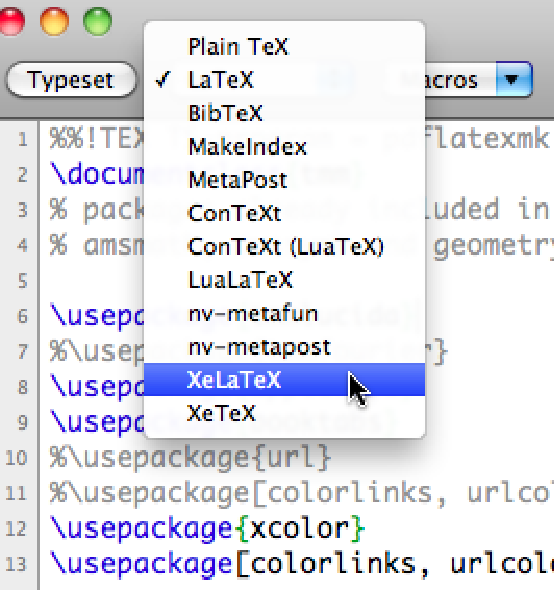
\includegraphics[width=2in]{figs/OriginalTypesetPopup}\qquad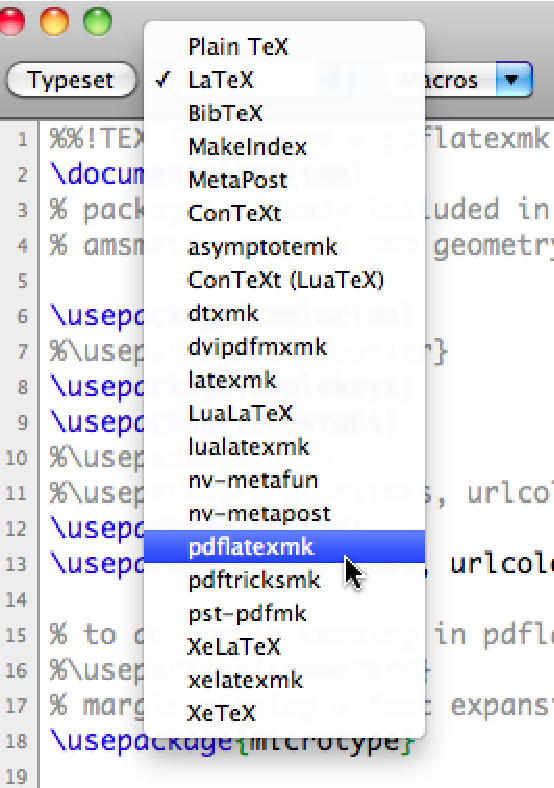
\includegraphics[width=2in]{figs/UpdatedTypesetPopup}
\caption{Default and updated versions of the engine pop-up menu after installing the \texttt{latexmk} engines.}\label{fig:popupmenus}
\end{figure}

Detailed information about using \texttt{latexmk} with the \texttt{epstopdf}, \texttt{pdftricks} and \texttt{pst-pdf} packages is discussed later.

I have only tested these engines with relatively trivial distributed documents (which include other files using \verb|\include| commands) but it appears that \texttt{latexmk} deals with them properly. Note that when compiling a file with name \texttt{rootname.tex} a file with name \texttt{rootname.fdb\_latexmk}\footnote{The dependency file had extension \texttt{dep} in previous versions of \texttt{latexmk} but didn't do a complete job of keeping track of those dependencies.} is created. This file contains the dependency information for the distributed document so making changes in an included file will force the recompile of the root document by \texttt{latexmk}.

%\section{Noteworthy Changes with \texttt{latexmk}.}
%
%Versions of \texttt{latexmk} prior to 3.21c weren't able to deal with the \texttt{glossary}, \texttt{glossaries} or \texttt{nomencl} packages because they re-write their output file(s) with each run of \texttt{(pdf/xe)latex} or use custom file extensions. This changed with \texttt{latexmk} 3.21c. The \texttt{latexmkrcedit}, generated the first time you run one of the new engines, is set to recognize the standard file extensions produced by the these packages and process them correctly and ``auto-magically.'' If you are creating custom glossaries or indexes you will have to properly edit the \texttt{latexmkrcedit} file found in the \path{~/Library/TeXShop/bin/} directory to add the dependencies; it should be fairly clear from the contents of that file what has to be added.
%
%Another major addition in \texttt{latexmk} since 3.21c is support for packages that create multiple bibliographies and/or indexes; e.g., when the \texttt{bibunits}, \texttt{chapterbib}, \texttt{multibib}, \texttt{multind} or similar packages are used. The extra processing needed for those packages happens automatically. Unfortunately, the \texttt{index} package uses the same naming scheme\footnote{Custom extensions rather than standard extensions with custom root file names.} as the \texttt{glossary} and \texttt{glossaries} packages (see the sub-section below) so you need to define extra dependencies and processing rules in the provided \texttt{rc} files. There was a bug in \texttt{latexmk} 3.21j that didn't allow it to work properly with the \texttt{index} package when creating an ordinary index (an \texttt{.idx} file); this was corrected with version 4.01 of \texttt{latexmk}.
%
%With \texttt{latexmk} 4.11 came three bug fixes:
%\begin{inparaenum}[i)]
%\item
%Corrected a bug with distributed documents using \texttt{bibtex} where changes in bibliography citations did not always trigger a rerun of \texttt{bibtex}.
%\item
%Fixed a problem when \texttt{latexmk} did not detect changed aux files, etc., on a small document when the run of \texttt{(xe/pdf)latex} was within the 1-second granularity of file times.
%\item
%Improved start-up times on some large documents by avoiding unnecessary recalculations of md5 checksums.
%\end{inparaenum}
%In particular, the last item seems to result in a very noticeable improvement in performance.
%
%\texttt{Latexmk} 4.12 adds one feature. If you have a \texttt{tex} file and an associated \texttt{bbl} file but \emph{not} the original \texttt{bib} file the \texttt{-bibitex-cond} option tells \texttt{latexmk} \emph{not} to run \texttt{bibtex} which would overwrite the \texttt{bbl} file with an empty bibliography. If the \texttt{bib} file is present and along the standard search path \texttt{latexmk} behaves identically to its previous versions. Versions 4.13 and 4.13a have now set this option as the default behavior. The 4.16 version of \texttt{latexmk} fixes a problem with misparsed log files in some versions of pdflatex and updates documentation to mention previously undocumented feature about the use of temporary files in making ps and pdf files. Version 4.16a fixed some bugs that don't effect its behavior under \TS.
%
\subsection{Using the \texttt{epstopdf} package with \texttt{latexmk}.}

%Including \texttt{eps} graphics files directly in \texttt{pdflatex} documents requires the use of the \texttt{epstopdf} package. If you have an included \texttt{eps} file \emph{and a converted \texttt{pdf} version of the file doesn't exist} the \texttt{epstopdf} package converts the \texttt{eps} file into a corresponding \texttt{pdf} file. 

%\subsubsection{Using \texttt{latexmk} with \texttt{epstopdf} version 1.4 and earlier.}

%With \texttt{epstopdf} versions 1.4 and earlier once the \texttt{pdf} image file exists the conversion no longer takes place \emph{even if the \texttt{eps} file is updated}. The \texttt{pdflatexmkrc} file now contains a dependency that uses a new rule, built into \texttt{latexmk} 4.01 and later, that will  delete a previously generated \texttt{pdf} file and then run \texttt{pdflatex} so that \texttt{epstopdf} will regenerate the \texttt{pdf} image file. \textbf{Note: The file name in your \texttt{\textbackslash includegraphics} commands should \emph{not} have an \texttt{eps} extension to prevent extra, unnecessary runs of \texttt{pdflatex}.}

%\subsubsection{Using \texttt{latexmk} with \texttt{epstopdf} version 1.5 and later.}

\subsubsection{A word about \MacTeX\ 2009 \& 2010}

% This is if embedded epstopdf in graphic(s/x) IS in MacTeX-2009
There are two changes to the graphics sub-system that first appear in \MacTeX\ 2009:
\begin{enumerate}
%\item
%The \texttt{graphic(s/x)} package now loads the \texttt{epstopdf} package when compiling with \texttt{pdflatex}. This is an attempt to make \texttt{eps} graphics inclusion under \texttt{pdflatex} a bit more transparent. (Note: This feature may not be present in the inital release of \MacTeX\ 2009.)
\item
The \texttt{epstopdf} package now defaults to using the \texttt{[update,append]} option. This has consequences if you don't use extensions when you include graphics files in your document.
\item
The default conversion is now \texttt{foo.eps}\,\(\to\)\,\texttt{foo-eps-converted-to.pdf}\footnote{This suffix can be customized.} to prevent any problems with overwriting a \texttt{foo.pdf} .
\end{enumerate}
The second of the changes to \texttt{epstopdf} leads to problems with \texttt{latexmk} version 4.08 and earlier since the base file name changes. To make the latest \texttt{epstopdf} operate properly with latexmk version 4.08 and earlier I suggest creating an \texttt{epstopdf.cfg} file, to be placed in \path{~/Library/texmf/tex/latex/config} and containing the line
\begin{verbatim}
\epstopdfsetup{update,prepend,prefersuffix=false,suffix=}
\end{verbatim}
making \texttt{epstopdf} behave as before; the conversion becomes \texttt{foo.eps}\,\(\to\)\,\texttt{foo.pdf}. Using \texttt{latexmk} version 4.10 or later requires no changes to \texttt{epstopdf} behavior but you may still do so if you wish to retain the pre-2009 behavior. You can find out the version number of the \texttt{latexmk} program you are using by running the command
\begin{verbatim}
~/Library/TeXShop/bin/tslatexmk/latexmk -v
\end{verbatim}
in \texttt{Terminal}.

Starting with \MacTeX\ 2010 the \texttt{graphic(x/s)} package will automatically load the \texttt{epstopdf} package if it detects that the file is being compiled using \texttt{pdftex} in \texttt{pdf} mode (normal for \texttt{pdflatex}). You no longer need to explicitly use the \texttt{epstopdf} package. Not only that but, if you haven't defined custom conversion and are only trying to convert \texttt{eps}\(\to\)\texttt{pdf} there isn't even a need to use the \texttt{--shell-escape} flag: edit the \texttt{latexmkrcedit} file to eliminate it from all of the engines.

% END of epstopdf embedded in graphic(s/x) IS in MacTeX-2009

% This is if epstopdf embedded in graphic(s/x) ISN'T in MacTeX-2009
%There are two changes\footnote{A third change, having the \texttt{graphic(s/x)} package automatically load the \texttt{epstopdf} package when compiling with \texttt{pdflatex}, as an attempt to make \texttt{eps} graphics inclusion under \texttt{pdflatex} a bit more transparent, has been postponed for the initial release of \MacTeX\ 2009. It may reappear in an update this coming year.
%} to the graphics sub-system that first appear in \MacTeX\ 2009:
%\begin{enumerate}
%\item
%The \texttt{epstopdf} package now defaults to using the \texttt{[update,append]} option. This has consequences if you don't use extensions when you include graphics files in your document.
%\item
%To prevent any problems with overwriting a \texttt{foo.pdf} the default conversion is now \texttt{foo.eps}\,\(\to\)\,\texttt{foo-eps-converted-to.pdf}\footnote{This suffix can be customized.}.
%\end{enumerate}
%The second of the changes to \texttt{epstopdf} leads to problems with \texttt{latexmk} version 4.08 and earlier since the base file name changes. To make the latest \texttt{epstopdf} operate properly with latexmk version 4.08 and earlier I suggest creating an \texttt{epstopdf.cfg} file which contains the line
%\begin{verbatim}
%\epstopdfsetup{update,prepend,prefersuffix=false,suffix=}
%\end{verbatim}
%to make \texttt{epstopdf} behave as before; the conversion becomes \texttt{foo.eps}\,\(\to\)\,\texttt{foo.pdf}. Using \texttt{latexmk} version 4.10 or later requires no changes to \texttt{epstopdf} behavior but you may still do so if you wish to retain the pre-2009 behavior. You can find out the version number of the \texttt{latexmk} program you are using by running the command
%\begin{verbatim}
%  ~/Library/TeXShop/bin/latexmk -v
%\end{verbatim}
%in \texttt{Terminal}.
% END of epstopdf embedded in graphic(s/x) ISN'T in MacTeX-2009

\subsubsection{Working with \texttt{epstopdf}.}

Versions of \texttt{epstopdf} from 1.5 on will automatically update a previously generated \texttt{pdf} file if the corresponding \texttt{eps} file is updated\footnote{Versions of \texttt{epstopdf} earlier than 1.5 never updated the \texttt{pdf} file once it existed.}. To let \texttt{latexmk} ``know'' that it should allow runs of \texttt{pdflatex} if the corresponding \texttt{eps} file is updated the necessary \texttt{rc} files (the ones that run \texttt{pdflatex} rather than \texttt{latex}; \texttt{pdflatexmkrc}, \texttt{pdftricksmkrc}, \texttt{pst-pdfmkrc} and \texttt{asymptotemkrc}) contain a special dependency and rule
\begin{verbatim}
add_cus_dep('eps', 'pdf', 0, 'cus_dep_require_primary_run');
\end{verbatim}
which passes \texttt{latexmk} the proper behavior.

If you are using \texttt{epstopdf} 1.5 or later with earlier \TeX\ distributions you should invoke it using the \texttt{[update,prepend]} options. For versions of \texttt{epstopdf} earlier than 1.5 you should edit the \texttt{pdflatexmkrc}, \texttt{pdftrcksmkrc}, \texttt{pst-pdfmkrc} and \texttt{asymptotemkrc} files by commenting out the original dependency (place a \texttt{\#} before the line
\begin{verbatim}
add_cus_dep('eps', 'pdf', 0, 'cus_dep_require_primary_run');
\end{verbatim}
in that file) and uncommenting the new dependency (remove the \texttt{\#} from the start of the line
\begin{verbatim}
#add_cus_dep('eps', 'pdf', 0, 'cus_dep_delete_dest');
\end{verbatim}
in that same file). This will have \texttt{latexmk} remove the \texttt{pdf} file before running \texttt{pdflatex} so \texttt{epstopdf} will recreate the \texttt{pdf} file. NOTE: These files may be automatically updated when \TS\ is updated and you may lose your changes!

%You can use the same (default with this distribution) processing with \texttt{epstopdf} 1.5 and later, however the \texttt{epstopdf} package, version 1.5 and later can check for an updated \texttt{eps} file and then recreate the \texttt{pdf} file if the \texttt{[update,prepend]} package options are used.  The dependency checking by \texttt{latexmk} is still important to let \texttt{latexmk} ``know'' that an included \texttt{eps} file has changed but the deletion of the \texttt{pdf} image file is unnecessary.  The \texttt{pdflatexmkrc}, etc., support files for \texttt{latexmk} 4.01 and later now contain a dependency and rule that will detect an updated \texttt{eps} file but let \texttt{epstopdf} do the conversion to \texttt{pdf}. By default this dependency is turned \emph{off} in \texttt{pdflatexmkrc}; to turn it on you should edit that file by commenting out the original dependency (place a \texttt{\#} before the line
%\begin{verbatim}
%add_cus_dep('eps', 'pdf', 0, 'cus_dep_delete_dest');
%\end{verbatim}
%in that file) and uncommenting the new dependency (remove the \texttt{\#} from the start of the line
%\begin{verbatim}
%#add_cus_dep('eps', 'pdf', 0, 'cus_dep_require_primary_run');
%\end{verbatim}
%in that same file). Remember that \texttt{latexmk} will work properly without making this change.

In version 1.5 and later of the \texttt{epstopdf} package you can also specify non-default processing for the \texttt{eps} to \texttt{pdf} conversion\footnote{The default processing uses the \texttt{epstopdf} command which, in turn, uses \texttt{ghostscript}.}. Since \texttt{latexmk} lets the \texttt{epstopdf} package to do all of the necessary processing of the \texttt{eps} file any customized processing defined in the \texttt{tex} source file will be used.

%\textbf{Note: I have noticed that there are times when including the \texttt{eps} extension in \texttt{\textbackslash includegraphics} still gives rise to additional runs of \texttt{pdflatex} so I still recommend you leave off the extension in \texttt{\textbackslash includegraphics} commands.}

\subsection{Using the \texttt{pdftricks} package with \texttt{latexmk}.}

The \texttt{pdftricks} package allows the inclusion of \texttt{pstricks} graphics in documents compiled with \texttt{pdflatex}. The package generates a file for each postscript figure included in the document. Each of those figure files is then processed to produce a \texttt{pdf} file containing a figure with a tight enclosing bounding box. The \texttt{pdftricksmk} engine included with this version of \texttt{latexmk} processes the original file, the figure files, etc., all only if they have changed. To use the engine place the line
\begin{verbatim}
% !TEX TS-program = pdftricksmk
\end{verbatim}
at the start of the file and Typeset the file. The processing steps for each of the figure files is \texttt{latex}\(\to\)\texttt{dvips}\(\to\)\texttt{ps2pdf}\(\to\)\texttt{pdfcrop} to ensure the proper bounding box is created for each figure. \textbf{NOTE: you must use the \texttt{[noshell]} option to the \texttt{pdftricks} package or \texttt{latexmk} will get into a run-on condition. All figure processing will be taken care of by \texttt{latexmk}.}

\subsection{Using the \texttt{pst-pdf} package with \texttt{latexmk}.}

The \texttt{pst-pdf} package also allows the inclusion of \texttt{pstricks} graphics in documents compiled with \texttt{pdflatex}. When the source file is compiled with \texttt{latex} a \texttt{dvi} file containing all of the figures is created. Further processing through the sequence \texttt{dvips}\(\to\)\texttt{ps2pdf}\(\to\)\texttt{pdfcrop} produces a single file that contains all of the figures with proper bounding boxes. A run of \texttt{pdflatex} on the source file then includes all of the figures previously generated. The \texttt{pst-pdfmk} engine takes care of all of the intermediate processing of the figures as well as the final run(s) of \texttt{pdflatex}, etc. To use the engine place the line
\begin{verbatim}
% !TEX TS-program = pst-pdfmk
\end{verbatim}
at the start of the file and Typeset the file.

\subsection{The \texttt{glossary}, \texttt{glossaries} and such packages.}

Packages that produce multiple and custom indexes, glossaries, etc., use one of two naming schemes for the multiple files they create:
\begin{enumerate}
\item
The first uses standard extensions but special files names for the generated files. \texttt{Latexmk} can keep track of changes in and ``knows'' how to process these files. The \texttt{multibib} and \texttt{multind} packages are examples that use this method.
\item
The second uses the source file name for the file but uses custom extensions to create the files. \texttt{Latexmk} needs ``help'' to know how to process these files in the form of dependencies and rules. Dependencies tell \texttt{latexmk} what the input and output extensions are and which rule to use to go from input to output. The \texttt{index}, \texttt{glossary} and \texttt{glossaries} packages are examples that use this second method.
\end{enumerate}

In addition, while the \texttt{glossaries} package supersedes the \texttt{glossary} package the order of the file extensions created by acronym and custom lists, processed by \texttt{makeindex} and then read in by subsequent runs of \texttt{(xe/pdf)latex} are reversed in the two packages. This latest version of \texttt{latexmk} configured for \TS\ works correctly for both packages. If you need to create your own custom lists see the examples in the \texttt{latexmkrcedit} file for creating dependancies and rules for \texttt{latexmk}.

\section{What these engines won't do, etc.}

There are many features of \texttt{latexmk} that aren't used in these simple \texttt{engine} files. See the documentation for \texttt{latexmk} in the supplied full distribution.

The placement of the \texttt{latexmk} program in \path{~/Library/TeXShop/bin/tslatexmk/} is non-standard; that directory is not on the standard path. It is possible to put the program in \path{/usr/local/bin/} or use the version of \texttt{latexmk} that is part of \MacTeX-2008 and later and it will then be usable from the command line. If you use the program in one of those locations you should modify the \texttt{engine} files to reflect the change in location.

The contents of the \texttt{rc} files corresponds to the the settings for commands for \TS\ on my system. They are simply text files. Please read the \texttt{latexmk} documentation before changing the contents.

%Because of the way \texttt{latexmk} gets the default path for \texttt{bib} files it will generate an inconsequential error message unless the \texttt{bib} file is in the same directory as the source file; the \texttt{bib} file will still be found by \texttt{bibtex} if it is along the standard path for \texttt{bib} files supplied by \texttt{kpsewhich}. To suppress the spurious error message the supplied \texttt{engine} files build a \emph{temporary} \texttt{BIBINPUTS} environment variable by appending the output of \verb'`kpsewhich --show-path=bib | sed -e "s/\!\!//g"`' to a possibly predefined \texttt{BIBINPUTS} variable. If there is a problem with long waits for searches over a network you can edit each of the \texttt{engine} files and customize the setting of the \texttt{BIBINPUTS} environment variable.

Finally, changes in \texttt{eps} files \emph{included in figures} created by the \texttt{pdftricks} or \texttt{pst-pdf} packages are \emph{not} detected by this packaging \texttt{latexmk} at this time. I hope to correct that problem at a later date.

\section{Update for \TS\ 2.18 (and later) with \MacTeX\ 2008 (ditto).}

The \texttt{rc} files for this version of \texttt{latexmk} for use with \TS\ have been updated to allow use of \texttt{synctex}, a \texttt{tex\(\leftrightarrow\)pdf} synchronization technology, with \texttt{\MacTeX-2008} and \TS\ 2.18. If you are using \texttt{\MacTeX-2007} or earlier \TeX\ distributions and the inconsequential error message about an unknown option bothers you, remove the \texttt{--synctex=1} options provided in the supplied \texttt{rc} files.

\section{Update for \TS\ 2.30 (and later).}

The \texttt{--file-line-error} flag has been set for all compiles in the basic \texttt{rc} files. \TS\ 2.30 and later uses the information provided by this flag to localise the location of compile errors when you use the \texttt{Go to Error} command.

\section{Update for \TS\ 2.32 (and later).}

Starting with \TS\ 2.32 when \TS\ is updated any updates to the files in the \path{~/Library/TeXShop/bin/tslatexmk/} folder will automatically be installed. Any changes directly made to those files will be lost. Most of the extra dependencies and rules that were common to all the \texttt{rc} files have been moved to the new \path{~/Library/TeXShop/bin/latexmkrcedit} file and all additional personal dependencies and rules should be moved to that file. The \texttt{latexmkrcedit} file will \emph{not} be updated automatically.

%\end{document}

\vspace{5pt plus 2pt minus 1pt}\noindent
Try it\dots\ I hope you like it.

\vspace{5pt plus 2pt minus 1pt}\noindent
Good Luck,\\
Herb Schulz\\
(\href{mailto:herbs2@mac.com}{herbs2@mac.com})

\end{document}
